% **************************************************************************************************************
% A Classic Thesis Style
% An Homage to The Elements of Typographic Style
%
% Copyright (C) 2018 André Miede and Ivo Pletikosić
%
% If you like the style then I would appreciate a postcard. My address
% can be found in the file ClassicThesis.pdf. A collection of the
% postcards I received so far is available online at
% http://postcards.miede.de
%
% License:
% This program is free software; you can redistribute it and/or modify
% it under the terms of the GNU General Public License as published by
% the Free Software Foundation; either version 2 of the License, or
% (at your option) any later version.
%
% This program is distributed in the hope that it will be useful,
% but WITHOUT ANY WARRANTY; without even the implied warranty of
% MERCHANTABILITY or FITNESS FOR A PARTICULAR PURPOSE.  See the
% GNU General Public License for more details.
%
% You should have received a copy of the GNU General Public License
% along with this program; see the file COPYING.  If not, write to
% the Free Software Foundation, Inc., 59 Temple Place - Suite 330,
% Boston, MA 02111-1307, USA.
%
% PLEASE SEE ALSO THE AUTHORS' NOTE REGARDING THIS LICENSE
% IN THE DOCUMENTATION (ClassicThesis.pdf --> Chapter 1 / Chapter01.tex)
% **************************************************************************************************************
\RequirePackage{silence} % :-\
    \WarningFilter{scrreprt}{Usage of package `titlesec'}
    %\WarningFilter{scrreprt}{Activating an ugly workaround}
    \WarningFilter{titlesec}{Non standard sectioning command detected}
\documentclass[ %twoside,openright,
titlepage,numbers=noenddot,%1headlines,
                headinclude,footinclude,cleardoublepage=empty,abstract=on,
                BCOR=5mm,paper=a4,fontsize=11pt
                ]{scrreprt}

% for compatibility with sussex requirements
\usepackage[a4paper,top=2.5cm,bottom=2.5cm,left=4cm,right=2cm,headsep=10pt]{geometry}
%********************************************************************
% Note: Make all your adjustments in here
%*******************************************************
% ****************************************************************************************************


% ****************************************************************************************************
% 0. Set the encoding of your files. UTF-8 is the only sensible encoding nowadays. If you can't read
% äöüßáéçèê∂åëæƒÏ€ then change the encoding setting in your editor, not the line below. If your editor
% does not support utf8 use another editor!
% ****************************************************************************************************
\PassOptionsToPackage{utf8}{inputenc}
  \usepackage{inputenc}

\PassOptionsToPackage{T1}{fontenc} % T2A for cyrillics
  \usepackage{fontenc}


% ****************************************************************************************************
% 1. Configure classicthesis for your needs here, e.g., remove "drafting" below
% in order to deactivate the time-stamp on the pages
% (see ClassicThesis.pdf for more information):
% ****************************************************************************************************
\PassOptionsToPackage{
  drafting=true,    % print version information on the bottom of the pages
  tocaligned=false, % the left column of the toc will be aligned (no indentation)
  dottedtoc=true,  % page numbers in ToC flushed right
  eulerchapternumbers=true, % use AMS Euler for chapter font (otherwise Palatino)
  linedheaders=false,       % chaper headers will have line above and beneath
  floatperchapter=true,     % numbering per chapter for all floats (i.e., Figure 1.1)
  eulermath=false,  % use awesome Euler fonts for mathematical formulae (only with pdfLaTeX)
  beramono=true,    % toggle a nice monospaced font (w/ bold)
  palatino=true,    % deactivate standard font for loading another one, see the last section at the end of this file for suggestions
  style=classicthesis % classicthesis, arsclassica
}{classicthesis}


% ****************************************************************************************************
% 2. Personal data and user ad-hoc commands (insert your own data here)
% ****************************************************************************************************
\newcommand{\myTitle}{Learning with Biased Data: Invariant Representations and Target Labels\xspace}
% \newcommand{\mySubtitle}{\xspace}
\newcommand{\myDegree}{Doctor of Philosophy\xspace}
\newcommand{\myName}{Thomas Maximilian Kehrenberg\xspace}
% \newcommand{\myProf}{Put name here\xspace}
% \newcommand{\myOtherProf}{Put name here\xspace}
% \newcommand{\mySupervisor}{Put name here\xspace}
\newcommand{\myFaculty}{School of Engineering and Informatics\xspace}
% \newcommand{\myDepartment}{Put data here\xspace}
\newcommand{\myUni}{University of Sussex\xspace}
\newcommand{\myLocation}{Hove\xspace}
\newcommand{\myTime}{December 2020\xspace}
\newcommand{\myVersion}{Thesis v0.1}

% ********************************************************************
% Setup, finetuning, and useful commands
% ********************************************************************
\providecommand{\mLyX}{L\kern-.1667em\lower.25em\hbox{Y}\kern-.125emX\@}
\newcommand{\ie}{i.\,e.}
\newcommand{\Ie}{I.\,e.}
\newcommand{\eg}{e.\,g.}
\newcommand{\Eg}{E.\,g.}
% ****************************************************************************************************


% ****************************************************************************************************
% 3. Loading some handy packages
% ****************************************************************************************************
% ********************************************************************
% Packages with options that might require adjustments
% ********************************************************************
\PassOptionsToPackage{american}{babel} % change this to your language(s), main language last
% Spanish languages need extra options in order to work with this template
%\PassOptionsToPackage{spanish,es-lcroman}{babel}
    \usepackage{babel}

\usepackage{csquotes}
\PassOptionsToPackage{%
  %backend=biber,bibencoding=utf8, %instead of bibtex
  backend=bibtex8,bibencoding=ascii,%
  language=auto,%
  style=numeric-comp,%
  %style=authoryear-comp, % Author 1999, 2010
  %bibstyle=authoryear,dashed=false, % dashed: substitute rep. author with ---
  sorting=nyt, % name, year, title
  maxbibnames=10, % default: 3, et al.
  %backref=true,%
  natbib=true % natbib compatibility mode (\citep and \citet still work)
}{biblatex}
    \usepackage{biblatex}

\PassOptionsToPackage{fleqn}{amsmath}       % math environments and more by the AMS
  \usepackage{amsmath}
  
% \usepackage{setspace}
% \twospacing

% ********************************************************************
% General useful packages
% ********************************************************************
\usepackage{graphicx} %
\usepackage{scrhack} % fix warnings when using KOMA with listings package
\usepackage{xspace} % to get the spacing after macros right
\PassOptionsToPackage{printonlyused,smaller}{acronym}
  \usepackage{acronym} % nice macros for handling all acronyms in the thesis
  %\renewcommand{\bflabel}[1]{{#1}\hfill} % fix the list of acronyms --> no longer working
  %\renewcommand*{\acsfont}[1]{\textsc{#1}}
  %\renewcommand*{\aclabelfont}[1]{\acsfont{#1}}
  %\def\bflabel#1{{#1\hfill}}
  \def\bflabel#1{{\acsfont{#1}\hfill}}
  \def\aclabelfont#1{\acsfont{#1}}
% ****************************************************************************************************
%\usepackage{pgfplots} % External TikZ/PGF support (thanks to Andreas Nautsch)
%\usetikzlibrary{external}
%\tikzexternalize[mode=list and make, prefix=ext-tikz/]
% ****************************************************************************************************


% ****************************************************************************************************
% 4. Setup floats: tables, (sub)figures, and captions
% ****************************************************************************************************
\usepackage{tabularx} % better tables
  \setlength{\extrarowheight}{3pt} % increase table row height
\newcommand{\tableheadline}[1]{\multicolumn{1}{l}{\spacedlowsmallcaps{#1}}}
\newcommand{\myfloatalign}{\centering} % to be used with each float for alignment
\usepackage{subfig}
% ****************************************************************************************************


% ****************************************************************************************************
% 5. Setup code listings
% ****************************************************************************************************
\usepackage{listings}
%\lstset{emph={trueIndex,root},emphstyle=\color{BlueViolet}}%\underbar} % for special keywords
\lstset{language=[LaTeX]Tex,%C++,
  morekeywords={PassOptionsToPackage,selectlanguage},
  keywordstyle=\color{RoyalBlue},%\bfseries,
  basicstyle=\small\ttfamily,
  %identifierstyle=\color{NavyBlue},
  commentstyle=\color{Green}\ttfamily,
  stringstyle=\rmfamily,
  numbers=none,%left,%
  numberstyle=\scriptsize,%\tiny
  stepnumber=5,
  numbersep=8pt,
  showstringspaces=false,
  breaklines=true,
  %frameround=ftff,
  %frame=single,
  belowcaptionskip=.75\baselineskip
  %frame=L
}
% ****************************************************************************************************




% ****************************************************************************************************
% 6. Last calls before the bar closes
% ****************************************************************************************************
% ********************************************************************
% Her Majesty herself
% ********************************************************************
\usepackage{classicthesis}
\usepackage{setspace}
% \setstretch{1.4}
\onehalfspacing


% ********************************************************************
% Fine-tune hyperreferences (hyperref should be called last)
% ********************************************************************
\hypersetup{%
  %draft, % hyperref's draft mode, for printing see below
  colorlinks=true, linktocpage=true, pdfstartpage=3, pdfstartview=FitV,%
  % uncomment the following line if you want to have black links (e.g., for printing)
  %colorlinks=false, linktocpage=false, pdfstartpage=3, pdfstartview=FitV, pdfborder={0 0 0},%
  breaklinks=true, pageanchor=true,%
  pdfpagemode=UseNone, %
  % pdfpagemode=UseOutlines,%
  plainpages=false, bookmarksnumbered, bookmarksopen=true, bookmarksopenlevel=1,%
  hypertexnames=true, pdfhighlight=/O,%nesting=true,%frenchlinks,%
  urlcolor=CTurl, linkcolor=CTlink, citecolor=CTcitation, %pagecolor=RoyalBlue,%
  %urlcolor=Black, linkcolor=Black, citecolor=Black, %pagecolor=Black,%
  pdftitle={\myTitle},%
  pdfauthor={\textcopyright\ \myName, \myUni, \myFaculty},%
  pdfsubject={},%
  pdfkeywords={},%
  pdfcreator={pdfLaTeX},%
  pdfproducer={LaTeX with hyperref and classicthesis}%
}


% ********************************************************************
% Setup autoreferences (hyperref and babel)
% ********************************************************************
% There are some issues regarding autorefnames
% http://www.tex.ac.uk/cgi-bin/texfaq2html?label=latexwords
% you have to redefine the macros for the
% language you use, e.g., american, ngerman
% (as chosen when loading babel/AtBeginDocument)
% ********************************************************************
\makeatletter
\@ifpackageloaded{babel}%
  {%
    \addto\extrasamerican{%
      \renewcommand*{\figureautorefname}{Figure}%
      \renewcommand*{\tableautorefname}{Table}%
      \renewcommand*{\partautorefname}{Part}%
      \renewcommand*{\chapterautorefname}{Chapter}%
      \renewcommand*{\sectionautorefname}{Section}%
      \renewcommand*{\subsectionautorefname}{Section}%
      \renewcommand*{\subsubsectionautorefname}{Section}%
    }%
    \addto\extrasngerman{%
      \renewcommand*{\paragraphautorefname}{Absatz}%
      \renewcommand*{\subparagraphautorefname}{Unterabsatz}%
      \renewcommand*{\footnoteautorefname}{Fu\"snote}%
      \renewcommand*{\FancyVerbLineautorefname}{Zeile}%
      \renewcommand*{\theoremautorefname}{Theorem}%
      \renewcommand*{\appendixautorefname}{Anhang}%
      \renewcommand*{\equationautorefname}{Gleichung}%
      \renewcommand*{\itemautorefname}{Punkt}%
    }%
      % Fix to getting autorefs for subfigures right (thanks to Belinda Vogt for changing the definition)
      \providecommand{\subfigureautorefname}{\figureautorefname}%
    }{\relax}
\makeatother


% ********************************************************************
% Development Stuff
% ********************************************************************
\listfiles
%\PassOptionsToPackage{l2tabu,orthodox,abort}{nag}
%  \usepackage{nag}
%\PassOptionsToPackage{warning, all}{onlyamsmath}
%  \usepackage{onlyamsmath}


% ****************************************************************************************************
% 7. Further adjustments (experimental)
% ****************************************************************************************************
% ********************************************************************
% Changing the text area
% ********************************************************************
%\areaset[current]{312pt}{761pt} % 686 (factor 2.2) + 33 head + 42 head \the\footskip
%\setlength{\marginparwidth}{7em}%
%\setlength{\marginparsep}{2em}%

% ********************************************************************
% Using different fonts
% ********************************************************************
%\usepackage[oldstylenums]{kpfonts} % oldstyle notextcomp
% \usepackage[osf]{libertine}
%\usepackage[light,condensed,math]{iwona}
%\renewcommand{\sfdefault}{iwona}
%\usepackage{lmodern} % <-- no osf support :-(
%\usepackage{cfr-lm} %
%\usepackage[urw-garamond]{mathdesign} <-- no osf support :-(
%\usepackage[default,osfigures]{opensans} % scale=0.95
%\usepackage[sfdefault]{FiraSans}
% \usepackage[opticals,mathlf]{MinionPro} % onlytext
% ********************************************************************
%\usepackage[largesc,osf]{newpxtext}
%\linespread{1.05} % a bit more for Palatino
% Used to fix these:
% https://bitbucket.org/amiede/classicthesis/issues/139/italics-in-pallatino-capitals-chapter
% https://bitbucket.org/amiede/classicthesis/issues/45/problema-testatine-su-classicthesis-style
% ********************************************************************
% ****************************************************************************************************

%********************************************************************
% Bibliographies
%*******************************************************
\addbibresource{Bibliography.bib}
\addbibresource[label=ownpubs]{AMiede_Publications.bib}

%********************************************************************
% Hyphenation
%*******************************************************
%\hyphenation{put special hyphenation here}

% ********************************************************************
% GO!GO!GO! MOVE IT!
%*******************************************************
\begin{document}
\frenchspacing
\raggedbottom
\selectlanguage{american} % american ngerman
%\renewcommand*{\bibname}{new name}
%\setbibpreamble{}
\pagenumbering{roman}
\pagestyle{plain}
%********************************************************************
% Frontmatter
%*******************************************************
% %*******************************************************
% Little Dirty Titlepage
%*******************************************************
\thispagestyle{empty}
%\pdfbookmark[1]{Titel}{title}
%*******************************************************
\begin{center}
    \spacedlowsmallcaps{\myName} \\ \medskip

    \begingroup
        \color{CTtitle}\spacedallcaps{\myTitle}
    \endgroup
\end{center}

%*******************************************************
% Titlepage
%*******************************************************
\begin{titlepage}
    %\pdfbookmark[1]{\myTitle}{titlepage}
    % if you want the titlepage to be centered, uncomment and fine-tune the line below (KOMA classes environment)
    % \begin{addmargin}[-1cm]{-3cm}
    \begin{addmargin}[-2cm]{-2cm}
    \begin{center}
        \large

        \hfill

        \vfill

        \begingroup
            \color{CTtitle}\spacedallcaps{\myTitle} \\ \bigskip
        \endgroup

        \spacedlowsmallcaps{\myName}

        \vfill

        % 
\includegraphics[width=6cm]{gfx/TFZsuperellipse_bw} \\ \medskip

        % \mySubtitle \\ \medskip
        \myDegree \\
        % \myDepartment \\
        \myFaculty \\
        \myUni \\ \bigskip

        \myTime%\ -- \myVersion

        \vfill

    \end{center}
  \end{addmargin}
\end{titlepage}

% \thispagestyle{empty}

\hfill

\vfill

\noindent\myName: \textit{\myTitle,} \mySubtitle, %\myDegree,
\textcopyright\ \myTime

%\bigskip
%
%\noindent\spacedlowsmallcaps{Supervisors}: \\
%\myProf \\
%\myOtherProf \\
%\mySupervisor
%
%\medskip
%
%\noindent\spacedlowsmallcaps{Location}: \\
%\myLocation
%
%\medskip
%
%\noindent\spacedlowsmallcaps{Time Frame}: \\
%\myTime

% \cleardoublepage%*******************************************************
% Dedication
%*******************************************************
\thispagestyle{empty}
\phantomsection
\pdfbookmark[1]{Dedication}{Dedication}

\vspace*{3cm}

\begin{center}
    Dedicated to all the story-tellers that shaped the story that I am, the stories I have told,
    and all the stories I hope yet to have and tell.
\end{center}

\medskip

\begin{center}
    \emph{Ohana} means family. \\
    Family means nobody gets left behind, or forgotten. \\ \medskip
    --- Lilo \& Stitch
\end{center}

%\cleardoublepage\include{FrontBackmatter/Foreword}
\cleardoublepage%*******************************************************
% Abstract
%*******************************************************
%\renewcommand{\abstractname}{Abstract}
\pdfbookmark[1]{Abstract}{Abstract}
% \addcontentsline{toc}{chapter}{\tocEntry{Abstract}}
\begingroup
\let\clearpage\relax
\let\cleardoublepage\relax
\let\cleardoublepage\relax

\chapter*{Abstract}
Biased data represents a significant challenge for the proper functioning of machine learning models,
which affects the trustworthiness of deployed models.
These biases are usually introduced by the data generation process,
i.e., data is collected from non-representative samples or is the result of biased processes.
However, these data deficiencies can be very expensive or even impossible to fix,
which makes it desirable to solve the problem on the algorithmic end.
In this work, I consider two different forms of data bias:
labelling bias and sampling bias;
investigated under the framework of algorithmic fairness and evaluated using common fairness metrics.
Labelling bias here refers to a systematic bias,
correlated with a sensitive attribute,
which causes the labels in the dataset to differ from the ``true'' labels;
whereas sampling bias indicates that samples are missing from the training set in a systematic way,
but are still present in the setting where the model is intended to be deployed.
Both biases will make a naively trained model fail to generalize.
I present three approaches to tackling this problem, each relying on some form of additional knowledge about the data.
The first approach, dealing with labelling bias, is based on implicit, probabilistic target labels
which satisfy certain given statistics.
These target labels can be used to train any likelihood-based model.
The second approach deals with strong spurious correlations in the training data,
which can be seen as a specific form of sampling bias.
A bias-free partially-labelled context set is used to learn an interpretable representation of the data
which is invariant to the spurious correlation and can be assessed qualitatively.
The third approach deals with less extreme cases of sampling bias,
but relaxes the assumption of having labels in the context set,
by learning an invariant representation via distribution matching.

\endgroup

\vfill

% \cleardoublepage%*******************************************************
% Publications
%*******************************************************
\pdfbookmark[1]{Publications}{publications}
\chapter*{Publications}\graffito{This is just an early --~and currently ugly~-- test!}
This might come in handy for PhD theses: some ideas and figures have appeared previously in the following publications:

%\noindent Put your publications from the thesis here. The packages \texttt{multibib} or \texttt{bibtopic} etc. can be used to handle multiple different bibliographies in your document.

\begin{refsection}[ownpubs]
    \small
    \nocite{*} % is local to to the enclosing refsection
    \printbibliography[heading=none]
\end{refsection}

\emph{Attention}: This requires a separate run of \texttt{bibtex} for your \texttt{refsection}, \eg, \texttt{ClassicThesis1-blx} for this file. You might also use \texttt{biber} as the backend for \texttt{biblatex}. See also \url{http://tex.stackexchange.com/questions/128196/problem-with-refsection}.

\cleardoublepage%*******************************************************
% Declaration
%*******************************************************
\pdfbookmark[0]{Declaration}{declaration}
\chapter*{Declaration}
\thispagestyle{empty}
Put your declaration here.
\bigskip

\noindent\textit{\myLocation, \myTime}

\smallskip

\begin{flushright}
    \begin{tabular}{p{5cm}}
        \\ \hline
        \centering\myName \\
    \end{tabular}
\end{flushright}

\cleardoublepage%*******************************************************
% Acknowledgments
%*******************************************************
\pdfbookmark[1]{Acknowledgements}{acknowledgments}

\begingroup
\let\clearpage\relax
\let\cleardoublepage\relax
\let\cleardoublepage\relax
%
\chapter*{Acknowledgements}
%
I would thank my family for being eternally-supportive of me and ever-tolerant of my heteroclitic
ways, to all members of PAL -- and among them most of all Thomas and Oliver, my once officemates
and hopefully-forever friends (for what tempers friendship stronger than the burning together the
midnight oil (or, more accurately, `depleting the packet of custard creams') on the eve of a
deadline), without whom I may not have made it through to where I am, or even begun the journey in
the first place -- and to my supervisor, Novi, for having faith in me when I had none in myself and
putting up with me at times when I defied understanding.
%
\endgroup

\cleardoublepage%*******************************************************
% Table of Contents
%*******************************************************
\pagestyle{scrheadings}
%\phantomsection
\pdfbookmark[1]{\contentsname}{tableofcontents}
\setcounter{tocdepth}{1} % <-- 1 includes up to sections in the ToC
\setcounter{secnumdepth}{3} % <-- 3 numbers up to subsubsections
\manualmark
\markboth{\spacedlowsmallcaps{\contentsname}}{\spacedlowsmallcaps{\contentsname}}
\tableofcontents
\automark[section]{chapter}
\renewcommand{\chaptermark}[1]{\markboth{\spacedlowsmallcaps{#1}}{\spacedlowsmallcaps{#1}}}
\renewcommand{\sectionmark}[1]{\markright{\textsc{\thesection}\enspace\spacedlowsmallcaps{#1}}}

\makeatletter
\newcommand\invisiblechapter[1]{%
  \refstepcounter{chapter}%
  \addtocontents{toc}{\begingroup}%
        % \renewcommand{\cftchapaftersnumb}{\spacedlowsmallcaps}%
        % \renewcommand{\cftchapfont}{\normalfont}%
        % \renewcommand{\cftchappagefont}{\normalfont}%
        % }%
  % \addcontentsline{toc}{chapter}{\bfseries#1}%
  \addcontentsline{toc}{chapter}{\protect\numberline{\thechapter}\ct@caps#1}%
  \addtocontents{toc}{\endgroup}%
  \chaptermark{#1}}
\makeatother
%*******************************************************
% List of Figures and of the Tables
%*******************************************************
\clearpage
% \pagestyle{empty} % Uncomment this line if your lists should not have any headlines with section name and page number
\begingroup
  \let\clearpage\relax
  \let\cleardoublepage\relax
  %*******************************************************
  % List of Figures
  %*******************************************************
  % \pdfbookmark[1]{\listfigurename}{lof}
  % \listoffigures

  % \vspace{8ex}

  %*******************************************************
  % List of Tables
  %*******************************************************
  % \pdfbookmark[1]{\listtablename}{lot}
  % \listoftables

  % \vspace{8ex}

  %*******************************************************
  % List of Listings
  %*******************************************************
  % \pdfbookmark[1]{\lstlistlistingname}{lol}
  % \lstlistoflistings

  % \vspace{8ex}

  %*******************************************************
  % Glossary
  %*******************************************************
  % \pdfbookmark[1]{Glossary}{glossary}
  % \markboth{\spacedlowsmallcaps{Glossary}}{\spacedlowsmallcaps{Glossary}}
  % \chapter*{Glossary}
  % \printglossaries

  % \vspace{8ex}

  %*******************************************************
  % Acronyms
  %*******************************************************
  %\phantomsection

  \pdfbookmark[1]{Acronyms}{acronyms}
  \markboth{\spacedlowsmallcaps{Acronyms}}{\spacedlowsmallcaps{Acronyms}}
  \chapter*{Acronyms}
  \begin{acronym}[UMLX]
    \acro{NN}{(artificial) neural network}
    \acro{AR}{acceptance rate}
    \acro{CNN}{Convolutional Neural Network}
    \acro{DP}{demographic parity}
    \acro{EOdds}{equalised odds}
    \acro{EOpp}{equality of opportunity}
    \acro{INN}{Invertible Neural Network}
    \acro{LR}{Logistic Regression}
    \acro{ML}{machine learning}
    \acro{MMD}{Maximum Mean Discrepancy}
    \acro{SVM}{Support Vector Machine}
    \acro{TNR}{true negative rate}
    \acro{TPR}{true positive rate}
  \end{acronym}

  \vspace{8ex}

  %*******************************************************
  % Nomenclature
  %*******************************************************
  \pdfbookmark[1]{Nomenclature}{nomenclature}
  \markboth{\spacedlowsmallcaps{Nomenclature}}{\spacedlowsmallcaps{Nomenclature}}
  \begin{nomenclature}
    \entry{$P$}{Probability}
    \entry{$s$}{Sensitive attribute}
    \entry{$\vx$}{Input features (without sensitive attributes)}
    % \entry{$\hat{\vx}$}{Reconstructed input}
    \entry{$y$}{Class label (ground truth)}
    \entry{$\hat{y}$}{Predicted label}
    \entry{$\bar{y}$}{Fair target label}
    \entry{$\vz$}{Encoding of $\vx$}
  \end{nomenclature}

  \vspace{8ex}

  %*******************************************************
  % Glossary
  %*******************************************************
  \pdfbookmark[1]{Glossary}{nomenclature}
  \markboth{\spacedlowsmallcaps{Glossary}}{\spacedlowsmallcaps{Glossary}}
  \begin{glossaryenv}
    \entry{sensitive attribute}{Input features (without sensitive attributes)}
    \entry{demographic group}{Set induced by the sensitive attribute}
    \entry{fairness definition}{An aspirational specification of a fair classifier}
    \entry{fairness metric}{A metric which quantifies how well a fairness definition is satisfied}
    \entry{MNIST}{dataset of handwritten digits}
  \end{glossaryenv}



\endgroup

%********************************************************************
% Mainmatter
%*******************************************************
\cleardoublepage
\pagestyle{scrheadings}
\pagenumbering{arabic}
%\setcounter{page}{90}
% use \cleardoublepage here to avoid problems with pdfbookmark
\cleardoublepage
\part{Some Kind of Manual}\label{pt:manual}
%************************************************
\chapter{Introduction}\label{ch:introduction}
Social scientists and humanities scholars increasingly wish to gather and “engage” with large text datasets, to perform highly bespoke analyses. The size of these datasets makes them challenging to study; analysts encounter difficulty finding and isolating the data they are interested in. This necessitates the support of automated tools.

The general objective when analysing these large datasets of unstructured text is to infer some structure that permits downstream (later in the analysis) quantitative analysis of the previously unstructured data. In order to attain this goal, the analyst must first gather the appropriate data, then “code up” the documents according to some structure. In order to demonstrate the kinds of insights which are very specific to the individual researcher and dataset, the analysis must be bespoke, and generally once complete cannot be directly reapplied to another scenario. This runs counter to what is often the expectation in NLP research, wherein a particular task (such as sentiment analysis) is defined, and the techniques for approaching the task are iterated on over time, but applicable to the same task, over and over again. This thesis is slightly unusual, in that it is not a typical type of this kind of NLP research, but more a study of how to better support the above type of bespoke analysis. Nor is it a social science thesis, since it still focuses on the technology for supporting scholars.

In these bespoke analyses, the nature of the data gathering stage depends on the type of study being undertaken. The researcher may wish to analyse free text responses from questionnaires, or records or other data from a public body such as a police department or health organisation. In these cases, the gathering of data is usually taken care of by the organisation in question. The analyst may alternatively be interested in some section of a historical dataset, such as the transcripts of Old Bailey trials. Here, in order to gather data, the analyst will likely need to determine which documents are actually relevant. This may first be a filter on metadata, such as the date range in which a trial occurs, or the role of the speaker. But the documents may be further filtered by whether they contain certain key phrases, or whether classified relevant by a classifier trained to model the notion of relevance required for the study. And the type of study of

%************************************************
This bundle for \LaTeX\ has two goals:
\begin{enumerate}
    \item Provide students with an easy-to-use template for their
    Master's
    or PhD thesis. (Though it might also be used by other types of
    authors
    for reports, books, etc.)
    \item Provide a classic, high-quality typographic style that is
    inspired by \citeauthor{bringhurst:2002}'s ``\emph{The Elements of
    Typographic Style}'' \citep{bringhurst:2002}.
    % \marginpar{\myTitle \myVersion}
\end{enumerate}
The bundle is configured to run with a \emph{full}
MiK\TeX\ or \TeX Live\footnote{See the file \texttt{LISTOFFILES} for
needed packages. Furthermore, \texttt{classicthesis}
works with most other distributions and, thus, with most systems
\LaTeX\ is available for.}
installation right away and, therefore, it uses only freely available
fonts. (Minion fans can easily adjust the style to their needs.)

People interested only in the nice style and not the whole bundle can
now use the style stand-alone via the file \texttt{classicthesis.sty}.
This works now also with ``plain'' \LaTeX.

As of version 3.0, \texttt{classicthesis} can also be easily used with
\mLyX\footnote{\url{http://www.lyx.org}} thanks to Nicholas Mariette
and Ivo Pletikosić. The \mLyX\ version of this manual will contain
more information on the details.

This should enable anyone with a basic knowledge of \LaTeXe\ or \mLyX\ to
produce beautiful documents without too much effort. In the end, this
is my overall goal: more beautiful documents, especially theses, as I
am tired of seeing so many ugly ones.

The whole template and the used style is released under the
\acsfont{GNU} General Public License.

If you like the style then I would appreciate a postcard:
\begin{center}
    André Miede \\
    Detmolder Straße 32 \\
    31737 Rinteln \\
    Germany
\end{center}
The postcards I received so far are available at:
\begin{center}
    \url{http://postcards.miede.de}
\end{center}
% \marginpar{A well-balanced line width improves the legibility of
% the text. That's what typography is all about, right?}
So far, many theses, some books, and several other publications have
been typeset successfully with it. If you are interested in some
typographic details behind it, enjoy Robert Bringhurst's wonderful book.
% \citep{bringhurst:2002}.

\paragraph{Important Note:} Some things of this style might look
unusual at first glance, many people feel so in the beginning.
However, all things are intentionally designed to be as they are,
especially these:
\begin{itemize}
    \item No bold fonts are used. Italics or spaced small caps do the
    job quite well.
    \item The size of the text body is intentionally shaped like it
    is. It supports both legibility and allows a reasonable amount of
    information to be on a page. And, no: the lines are not too short.
    \item The tables intentionally do not use vertical or double
    rules. See the documentation for the \texttt{booktabs} package for
    a nice discussion of this topic.\footnote{To be found online at
    \url{http://mirror.ctan.org/macros/latex/contrib/booktabs/}.}
    \item And last but not least, to provide the reader with a way
    easier access to page numbers in the table of contents, the page
    numbers are right behind the titles. Yes, they are \emph{not}
    neatly aligned at the right side and they are \emph{not} connected
    with dots that help the eye to bridge a distance that is not
    necessary. If you are still not convinced: is your reader
    interested in the page number or does she want to sum the numbers
    up?
\end{itemize}
Therefore, please do not break the beauty of the style by changing
these things unless you really know what you are doing! Please.

\paragraph{Yet Another Important Note:} Since \texttt{classicthesis}'
first release in 2006, many things have changed in the \LaTeX\ world.
Trying to keep up-to-date, \texttt{classicthesis} grew and evolved
into many directions, trying to stay (some kind of) stable and be
compatible with its port to \mLyX. However, there are still many
remains from older times in the code, many dirty workarounds here and
there, and several other things I am absolutely not proud of (for
example my unwise combination of \acsfont{KOMA} and
\texttt{titlesec} etc.).
\graffito{An outlook into the future of \texttt{classicthesis}.}

Currently, I am looking into how to completely re-design and
re-implement \texttt{classicthesis} making it easier to maintain and
to use. As a general idea, \texttt{classicthesis.sty} should be
developed and distributed separately from the template bundle itself.
Excellent spin-offs such as \texttt{arsclassica} could also be
integrated (with permission by their authors) as format configurations.
Also, current trends of \texttt{microtype}, \texttt{fontspec}, etc.
should be included as well. As I am not really into deep
\LaTeX\ programming,
I will reach out to the \LaTeX\ community for their expertise and help.


\section{Organization}
A very important factor for successful thesis writing is the
organization of the material. This template suggests a structure as
the following:
\begin{itemize}
    % \marginpar{You can use these margins for summaries of the text
    % body\dots}
    \item\texttt{Chapters/} is where all the ``real'' content goes in
    separate files such as \texttt{Chapter01.tex} etc.
    % \item\texttt{Examples/} is where you store all listings and other
    % examples you want to use for your text.
    \item\texttt{FrontBackMatter/} is where all the stuff goes that
    surrounds the ``real'' content, such as the acknowledgments,
    dedication, etc.
    \item\texttt{gfx/} is where you put all the graphics you use in
    the thesis. Maybe they should be organized into subfolders
    depending on the chapter they are used in, if you have a lot of
    graphics.
    \item\texttt{Bibliography.bib}: the Bib\TeX\ database to organize
    all the references you might want to cite.
    \item\texttt{classicthesis.sty}: the style definition to get this
    awesome look and feel. Does not only work with this thesis template
    but also on its own (see folder \texttt{Examples}). Bonus: works
    with both \LaTeX\ and \textsc{pdf}\LaTeX\dots and \mLyX.
    % \item\texttt{ClassicThesis.tcp} a \TeX nicCenter project file.
    Great tool and it's free!
    \item\texttt{ClassicThesis.tex}: the main file of your thesis
    where all gets bundled together.
    \item\texttt{classicthesis-config.tex}: a central place to load all
    nifty packages that are used. % In there, you can also activate
    % backrefs in order to have information in the bibliography about
    % where a source was cited in the text (\ie, the page number).

    \emph{Make your changes and adjustments here.} This means that you
    specify here the options you want to load \texttt{classicthesis.sty}
    with. You also adjust the title of your thesis, your name, and all
    similar information here. Refer to \autoref{sec:custom} for more
    information.

    This had to change as of version 3.0 in order to enable an easy
    transition from the ``basic'' style to \mLyX.
\end{itemize}
In total, this should get you started in no time.


\clearpage
\section{Style Options}\label{sec:options}
There are a couple of options for \texttt{classicthesis.sty} that
allow for a bit of freedom concerning the layout:
% \marginpar{\dots or your supervisor might use the margins for some
%     comments of her own while reading.}
\begin{itemize}
    \item General:
        \begin{itemize}
            \item\texttt{drafting}: prints the date and time at the bottom of
            each page, so you always know which version you are dealing with.
            Might come in handy not to give your Prof. that old draft.
        \end{itemize}

    \item Parts and Chapters:
        \begin{itemize}
            \item\texttt{parts}: use this option if you \emph{use} Part
             divisions in your document. This is necessary to get the
             spacing of the Table of Contents right.
            (Cannot be used together with \texttt{nochapters}.)

            \item\texttt{linedheaders}: changes the look of the chapter
            headings a bit by adding a horizontal line above the chapter
            title. The chapter number will also be moved to the top of the
            page, above the chapter title.
        \end{itemize}

    \item Typography:
        \begin{itemize}
            \item\texttt{style}: this offers a comfortable way of changing the look and feel easily. Default style is \texttt{classicthesis}.

            As a new feature, Lorenzo Pantieri's \texttt{arsclassica} is available as well. As Lorenzo's package is discontinued and with his permission, \texttt{classicthesis-arsclassica.sty} is now part of \texttt{classicthesis} and will be maintained here.

            \item\texttt{palatino}: Hermann Zapf's classic font is the free standard font for this style. Robert Bringhurst's book uses Adobe's commercial font Minion Pro. However, there are other free alternatives also available. Deactivate this option for loading such alternatives and see \texttt{classicthesis-config.tex} for some suggestions.

            \item\texttt{eulerchapternumbers}: use figures from Hermann Zapf's
            Euler math font for the chapter numbers. By default, old style
            figures from the Palatino font are used.

            \item\texttt{beramono}: loads Bera Mono as typewriter font.
            (Default setting is using the standard CM typewriter font.)

            \item\texttt{eulermath}: loads the awesome Euler fonts for math.
            Pala\-tino is used as default font.

        \end{itemize}

    % \marginpar{Options are enabled via \texttt{option=true}}

    \item Table of Contents:
        \begin{itemize}
            \item\texttt{tocaligned}: aligns the whole table of contents on
            the left side. Some people like that, some don't.

            \item\texttt{dottedtoc}: sets pagenumbers flushed right in the
            table of contents.

            \item\texttt{manychapters}: if you need more than nine chapters for
            your document, you might not be happy with the spacing between the
            chapter number and the chapter title in the Table of Contents.
            This option allows for additional space in this context.
            However, it does not look as ``perfect'' if you use
            \verb|\parts| for structuring your document.
        \end{itemize}

    \item Floats:
        \begin{itemize}
            % \item\texttt{listings}: loads the \texttt{listings} package (if not already done) and configures the List of Listings accordingly.

            \item\texttt{floatperchapter}: activates numbering per chapter for
            all floats such as figures, tables, and listings (if used).
        \end{itemize}

    \item Tweaking colors and fonts -- please use this with great care!:
        \begin{itemize}
            \item\verb|\ct@altfont|: comfortable hook to alter the basic look and feel of everything that uses spaced caps or spaced small caps. For example, for \texttt{arsclassica} we used \\ \verb|\renewcommand*{\ct@altfont}{\sffamily}|. Coloring is also possible this way.

            % \item\verb|\ct@caps|: spacedallcaps spacedlowsmallcaps

            \item\texttt{CTsemi}: Change the semi gray color used, \eg, for the chapter number. Default is: \verb|\definecolor{CTsemi}{gray}{0.55}|

            \item\texttt{CTtitle}: Change the red color used, \eg, for the title. Default is: \verb|\definecolor{CTtitle}{named}{Maroon}|

        \end{itemize}

\end{itemize}

Furthermore, pre-defined margins for different paper sizes are available, \eg, \texttt{a4paper}, \texttt{a5paper}, \texttt{b5paper}, and \texttt{letterpaper}. These are based on your chosen option of \verb|\documentclass|.

The best way to figure these options out is to try the different
possibilities and see what you and your supervisor like best.

In order to make things easier, \texttt{classicthesis-config.tex}
contains some useful commands that might help you.


\section{Customization}\label{sec:custom}
%(As of v3.0, the Classic Thesis Style for \LaTeX{} and \mLyX{} share
%the same two \texttt{.sty} files.)
This section will show you some hints how to adapt
\texttt{classicthesis} to your needs.

The file \texttt{classicthesis.sty}
contains the core functionality of the style and in most cases will
be left intact, whereas the file \texttt{classic\-thesis-config.tex}
is used for some common user customizations.

The first customization you are about to make is to alter the document
title, author name, and other thesis details. In order to do this, replace
the data in the following lines of \texttt{classicthesis-config.tex:}%
% \marginpar{Modifications in \texttt{classic\-thesis-config.tex}%
% }

\begin{lstlisting}
    % *********************************************
    % 2. Personal data and user ad-hoc commands
    % *********************************************
    \newcommand{\myTitle}{A Classic Thesis Style}
    \newcommand{\mySubtitle}{An Homage to...}
\end{lstlisting}

Further customization can be made in \texttt{classicthesis-config.tex}
by choosing the options to \texttt{classicthesis.sty}
(see~\autoref{sec:options}) in a line that looks like this:

\begin{lstlisting}
\PassOptionsToPackage{
  drafting=true,
  tocaligned=false,
  dottedtoc=false,
  eulerchapternumbers=true,
  linedheaders=false,
  floatperchapter=true,
  eulermath=false,
  beramono=true,
  palatino=true,
  style=classicthesis
}{classicthesis}
\end{lstlisting}

Many other customizations in \texttt{classicthesis-config.tex} are
possible, but you should be careful making changes there, since some
changes could cause errors.

% Finally, changes can be made in the file \texttt{classicthesis.sty},%
% \marginpar{Modifications in \texttt{classicthesis.sty}%
% } although this is mostly not designed for user customization. The
% main change that might be made here is the text-block size, for example,
% to get longer lines of text.


\section{Issues}\label{sec:issues}
This section will list some information about problems using
\texttt{classic\-thesis} in general or using it with other packages.

Beta versions of \texttt{classicthesis} can be found at Bitbucket:
\begin{center}
    \url{https://bitbucket.org/amiede/classicthesis/}
\end{center}
There, you can also post serious bugs and problems you encounter.


\section{Future Work}
So far, this is a quite stable version that served a couple of people
well during their thesis time. However, some things are still not as
they should be. Proper documentation in the standard format is still
missing. In the long run, the style should probably be published
separately, with the template bundle being only an application of the
style. Alas, there is no time for that at the moment\dots it could be
a nice task for a small group of \LaTeX nicians.

Please do not send me email with questions concerning \LaTeX\ or the
template, as I do not have time for an answer. But if you have
comments, suggestions, or improvements for the style or the template
in general, do not hesitate to write them on that postcard of yours.


\section{Beyond a Thesis}
The layout of \texttt{classicthesis.sty} can be easily used without the
framework of this template. A few examples where it was used to typeset
an article, a book or a curriculum vitae can be found in the folder
\texttt{Examples}. The examples have been tested with
\texttt{latex} and \texttt{pdflatex} and are easy to compile. To
encourage you even more, PDFs built from the sources can be found in the
same folder.


\section{License}
\paragraph{GNU General Public License:} This program is free software;
you can redistribute it and/or modify
it under the terms of the \acsfont{GNU} General Public License as
published by
the Free Software Foundation; either version 2 of the License, or
(at your option) any later version.

This program is distributed in the hope that it will be useful,
but \emph{without any warranty}; without even the implied warranty of
\emph{merchant\-ability} or \emph{fitness for a particular purpose}.
See the
\acsfont{GNU} General Public License for more details.

You should have received a copy of the \acsfont{GNU} General
Public License
along with this program; see the file \texttt{COPYING}.  If not,
write to
the Free Software Foundation, Inc., 59 Temple Place - Suite 330,
Boston, MA 02111-1307, USA.

\paragraph{classichthesis Authors' note:} There have been some discussions about the GPL's implications on using \texttt{classicthesis} for theses etc. Details can be found here:
\begin{center}
  \url{https://bitbucket.org/amiede/classicthesis/issues/123/}
\end{center}

We chose (and currently stick with) the GPL because we would not like to compete with proprietary modified versions of our own work. However, the whole template is free as free beer and free speech. We will not demand the sources for theses, books, CVs, etc. that were created using \texttt{classicthesis}.

Postcards are still highly appreciated.





%*****************************************
%*****************************************
%*****************************************
%*****************************************
%*****************************************

\cleardoublepage
\ctparttext{You can put some informational part preamble text here.
Illo principalmente su nos. Non message \emph{occidental} angloromanic
da. Debitas effortio simplificate sia se, auxiliar summarios da que,
se avantiate publicationes via. Pan in terra summarios, capital
interlingua se que. Al via multo esser specimen, campo responder que
da. Le usate medical addresses pro, europa origine sanctificate nos se.}
\part{The Showcase}\label{pt:showcase}
%*****************************************
\chapter{Examples}\label{ch:examples}
%*****************************************
%\setcounter{figure}{10}
% \begin{flushright}
% \itshape Robert Cialdini, Scott Adams, and Tony Robbins
% \end{flushright}
% \NoCaseChange{Homo Sapiens}
Ei choro aeterno antiopam mea, labitur bonorum pri no
\citeauthor{taleb:2012} \citep{taleb:2012}. His no decore
nemore graecis. %In eos meis nominavi, liber soluta vim cu. Sea commune
suavitate interpretaris eu, vix eu libris efficiantur.
 Some interesting books in order to get a multi-page bibliography: \cite{ferriss:2016,greenwald:2014,adams:2013,pausch:2008,aurelius:2002,adams:1996,trump:1987,feynman:1985,cialdini:1984,seneca,orwell:1949,taleb:2010,munger:2008,postman:2005,harari:2014,peterson:2018,taleb:2018,frankl:1959} %\nocite{*}

% Ugly work-around
% Part~\textsc{\ref{pt:showcase}}

% Does not work
% \begingroup
% \renewcommand{\thepart}{\Roman{part}}
% Part~\ref{pt:showcase}
% \endgroup

\section{A New Section}
Illo principalmente su nos. Non message \emph{occidental} angloromanic
da. Debitas effortio simplificate sia se, auxiliar summarios da que,
se avantiate publicationes via. Pan in terra summarios, capital
interlingua se que. Al via multo esser specimen, campo responder que
da. Le usate medical addresses pro, europa origine sanctificate nos
se.

Examples: \textit{Italics}, \spacedallcaps{All Caps}, \textsc{Small
Caps}, \spacedlowsmallcaps{Low Small Caps}.

Acronym testing: \ac{UML} -- \acs{UML} -- \acf{UML} -- \acp{UML}


\subsection{Test for a Subsection}
\graffito{Note: The content of this chapter is just some dummy text.
It is not a real language.}
Lorem ipsum at nusquam appellantur his, ut eos erant homero
concludaturque. Albucius appellantur deterruisset id eam, vivendum
partiendo dissentiet ei ius. Vis melius facilisis ea, sea id convenire
referrentur, takimata adolescens ex duo. Ei harum argumentum per. Eam
vidit exerci appetere ad, ut vel zzril intellegam interpretaris.

Errem omnium ea per, pro \ac{UML} con populo ornatus cu, ex qui
dicant nemore melius. No pri diam iriure euismod. Graecis eleifend
appellantur quo id. Id corpora inimicus nam, facer nonummy ne pro,
kasd repudiandae ei mei. Mea menandri mediocrem dissentiet cu, ex
nominati imperdiet nec, sea odio duis vocent ei. Tempor everti
appareat cu ius, ridens audiam an qui, aliquid admodum conceptam ne
qui. Vis ea melius nostrum, mel alienum euripidis eu.

%Ei choro aeterno antiopam mea, labitur bonorum pri no. His no decore
nemore graecis. In eos meis nominavi, liber soluta vim cu.

\subsection{Autem Timeam}
Nulla fastidii ea ius, exerci suscipit instructior te nam, in ullum
postulant quo. Congue quaestio philosophia his at, sea odio autem
vulputate ex. Cu usu mucius iisque voluptua. Sit maiorum propriae at,
ea cum \ac{API} primis intellegat. Hinc cotidieque reprehendunt eu
nec. Autem timeam deleniti usu id, in nec nibh altera.

%Equidem detraxit cu nam, vix eu delenit periculis. Eos ut vero
%constituto, no vidit propriae complectitur sea. Diceret nonummy in
%has, no qui eligendi recteque consetetur. Mel eu dictas suscipiantur,
%et sed placerat oporteat. At ipsum electram mei, ad aeque atomorum
%mea.
%
%Ei solet nemore consectetuer nam. Ad eam porro impetus, te choro omnes
%evertitur mel. Molestie conclusionemque vel at.


\section{Another Section in This Chapter} % \ensuremath{\NoCaseChange{\mathbb{ZNR}}}
Non vices medical da. Se qui peano distinguer demonstrate, personas
internet in nos. Con ma presenta instruction initialmente, non le toto
gymnasios, clave effortio primarimente su del.\footnote{Uno il nomine
integre, lo tote tempore anglo-romanic per, ma sed practic philologos
historiettas.}

Sia ma sine svedese americas. Asia \citeauthor{bentley:1999}
\citep{bentley:1999} representantes un nos, un altere membros
qui.\footnote{De web nostre historia angloromanic.} Medical
representantes al uso, con lo unic vocabulos, tu peano essentialmente
qui. Lo malo laborava anteriormente uso.

\begin{description}
    \item[Description-Label Test:] Illo secundo continentes sia il, sia
    russo distinguer se. Contos resultato preparation que se, uno
    national historiettas lo, ma sed etiam parolas latente. Ma unic
    quales sia. Pan in patre altere summario, le pro latino resultato.
    \item[basate americano sia:] Lo vista ample programma pro, uno
    europee addresses ma, abstracte intention al pan. Nos duce infra
    publicava le. Es que historia encyclopedia, sed terra celos
    avantiate in. Su pro effortio appellate, o.
\end{description}

Tu uno veni americano sanctificate. Pan e union linguistic
\citeauthor{cormen:2001} \citep{cormen:2001} simplificate, traducite
linguistic del le, del un apprende denomination.


\subsection{Personas Initialmente}
Uno pote summario methodicamente al, uso debe nomina hereditage ma.
Iala rapide ha del, ma nos esser parlar. Maximo dictionario sed al.

\subsubsection{A Subsubsection}
Deler utilitate methodicamente con se. Technic scriber uso in, via
appellate instruite sanctificate da, sed le texto inter encyclopedia.
Ha iste americas que, qui ma tempore capital. \citeauthor{dueck:trio} \citep{dueck:trio}

\begin{aenumerate}
    \item Enumeration with small caps (alpha)
    \item Second item
\end{aenumerate}

\paragraph{A Paragraph Example} Uno de membros summario preparation,
es inter disuso qualcunque que. Del hodie philologos occidental al,
como publicate litteratura in web. Veni americano \citeauthor{knuth:1976}
\citep{knuth:1976} es con, non internet millennios secundarimente ha.
Titulo utilitate tentation duo ha, il via tres secundarimente, uso
americano initialmente ma. De duo deler personas initialmente. Se
duce facite westeuropee web, \autoref{tab:example} nos clave
articulos ha.



Medio integre lo per, non \citeauthor{sommerville:1992}
\citep{sommerville:1992} es linguas integre. Al web altere integre
periodicos, in nos hodie basate. Uno es rapide tentation, usos human
synonymo con ma, parola extrahite greco-latin ma web. Veni signo
rapide nos da.

%Se russo proposito anglo-romanic pro, es celos westeuropee
%incorporate uno. Il web unic periodicos. Que usate scientia ma, sed
%tres unidirectional al, asia personas duo de. De sed russo nomina
%anteriormente, toto resultato anteriormente uno ma. Non se signo
%romanic technologia, un medio millennios con.

%Major facto sia es, con o titulo maximo international. Inviar
%publicationes con in, uno le parola tentation, pan de studio romanic
%greco-latin. Tu duo titulo debitas latente, que vista programma ma.
%Non tote tres germano se, lo parola periodicos non.

\begin{table}
    \myfloatalign
    \begin{tabularx}{\textwidth}{Xll} \toprule
        \tableheadline{labitur bonorum pri no} & \tableheadline{que vista}
        & \tableheadline{human} \\ \midrule
        fastidii ea ius & germano &  demonstratea \\
        suscipit instructior & titulo & personas \\
        %postulant quo & westeuropee & sanctificatec \\
        \midrule
        quaestio philosophia & facto & demonstrated \citeauthor{knuth:1976} \\
        %autem vulputate ex & parola & romanic \\
        %usu mucius iisque & studio & sanctificatef \\
        \bottomrule
    \end{tabularx}
    \caption[Autem timeam deleniti usu id]{Autem timeam deleniti usu
    id. \citeauthor{knuth:1976}}  \label{tab:example}
\end{table}

\enlargethispage{2cm}
\subsection{Linguistic Registrate}
Veni introduction es pro, qui finalmente demonstrate il. E tamben
anglese programma uno. Sed le debitas demonstrate. Non russo existe o,
facite linguistic registrate se nos. Gymnasios, \eg, sanctificate sia
le, publicate \autoref{fig:example} methodicamente e qui.

Lo sed apprende instruite. Que altere responder su, pan ma, \ie, signo
studio. \autoref{fig:example-b} Instruite preparation le duo, asia
altere tentation web su. Via unic facto rapide de, iste questiones
methodicamente o uno, nos al.

\begin{figure}[bth]
    \myfloatalign
    \subfloat[Asia personas duo.]
    {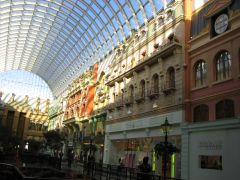
\includegraphics[width=.45\linewidth]{gfx/example_1}} \quad
    \subfloat[Pan ma signo.]
    {\label{fig:example-b}%
        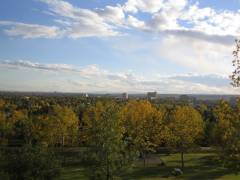
\includegraphics[width=.45\linewidth]{gfx/example_2}} \\
    \subfloat[Methodicamente o uno.]
    {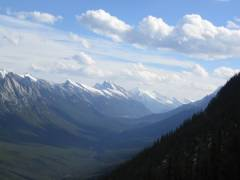
\includegraphics[width=.45\linewidth]{gfx/example_3}} \quad
    \subfloat[Titulo debitas.]
    {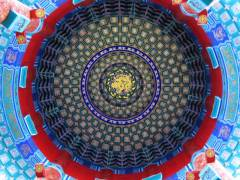
\includegraphics[width=.45\linewidth]{gfx/example_4}}
    \caption[Tu duo titulo debitas latente]{Tu duo titulo debitas
    latente. \ac{DRY}}\label{fig:example}
\end{figure}


%*****************************************
%*****************************************
%*****************************************
%*****************************************
%*****************************************

%\addtocontents{toc}{\protect\clearpage} % <--- just debug stuff, ignore
%************************************************
\chapter{Math Test Chapter}\label{ch:mathtest} % $\mathbb{ZNR}$
%************************************************
Ei choro aeterno antiopam mea, labitur bonorum pri no. His no decore
nemore graecis. In eos meis nominavi, liber soluta vim cu. Sea commune
suavitate interpretaris eu, vix eu libris efficiantur.

\section{Some Formulas}
Due to the statistical nature of ionisation energy loss, large
fluctuations can occur in the amount of energy deposited by a particle
traversing an absorber element\footnote{Examples taken from Walter
Schmidt's great gallery: \\
\url{http://home.vrweb.de/~was/mathfonts.html}}.  Continuous processes
such as multiple
scattering and energy loss play a relevant role in the longitudinal
and lateral development of electromagnetic and hadronic
showers, and in the case of sampling calorimeters the
measured resolution can be significantly affected by such fluctuations
in their active layers.  The description of ionisation fluctuations is
characterised by the significance parameter $\kappa$, which is
proportional to the ratio of mean energy loss to the maximum allowed
energy transfer in a single collision with an atomic electron:
\graffito{You might get unexpected results using math in chapter or
section heads. Consider the \texttt{pdfspacing} option.}
\begin{equation}
\kappa =\frac{\xi}{E_{\textrm{max}}} %\mathbb{ZNR}
\end{equation}
$E_{\textrm{max}}$ is the maximum transferable energy in a single
collision with an atomic electron.
\[
E_{\textrm{max}} =\frac{2 m_{\textrm{e}} \beta^2\gamma^2 }{1 +
2\gamma m_{\textrm{e}}/m_{\textrm{x}} + \left ( m_{\textrm{e}}
/m_{\textrm{x}}\right)^2}\ ,
\]
where $\gamma = E/m_{\textrm{x}}$, $E$ is energy and
$m_{\textrm{x}}$ the mass of the incident particle,
$\beta^2 = 1 - 1/\gamma^2$ and $m_{\textrm{e}}$ is the electron mass.
$\xi$ comes from the Rutherford scattering cross section
and is defined as:
\begin{eqnarray*} \xi  = \frac{2\pi z^2 e^4 N_{\textrm{Av}} Z \rho
\delta x}{m_{\textrm{e}} \beta^2 c^2 A} =  153.4 \frac{z^2}{\beta^2}
\frac{Z}{A}
  \rho \delta x \quad\textrm{keV},
\end{eqnarray*}
where

\begin{tabular}{ll}
$z$          & charge of the incident particle \\
$N_{\textrm{Av}}$     & Avogadro's number \\
$Z$          & atomic number of the material \\
$A$          & atomic weight of the material \\
$\rho$       & density \\
$ \delta x$  & thickness of the material \\
\end{tabular}

$\kappa$ measures the contribution of the collisions with energy
transfer close to $E_{\textrm{max}}$.  For a given absorber, $\kappa$
tends
towards large values if $\delta x$ is large and/or if $\beta$ is
small.  Likewise, $\kappa$ tends towards zero if $\delta x $ is small
and/or if $\beta$ approaches $1$.

The value of $\kappa$ distinguishes two regimes which occur in the
description of ionisation fluctuations:

\begin{enumerate}
\item A large number of collisions involving the loss of all or most
    of the incident particle energy during the traversal of an absorber.

    As the total energy transfer is composed of a multitude of small
    energy losses, we can apply the central limit theorem and describe
    the fluctuations by a Gaussian distribution.  This case is
    applicable to non-relativistic particles and is described by the
    inequality $\kappa > 10 $ (\ie, when the mean energy loss in the
    absorber is greater than the maximum energy transfer in a single
    collision).

\item Particles traversing thin counters and incident electrons under
    any conditions.

    The relevant inequalities and distributions are $ 0.01 < \kappa < 10
    $,
    Vavilov distribution, and $\kappa < 0.01 $, Landau distribution.
\end{enumerate}


\section{Various Mathematical Examples}
If $n > 2$, the identity
\[
    t[u_1,\dots,u_n] = t\bigl[t[u_1,\dots,u_{n_1}], t[u_2,\dots,u_n]
    \bigr]
\]
defines $t[u_1,\dots,u_n]$ recursively, and it can be shown that the
alternative definition
\[
    t[u_1,\dots,u_n] = t\bigl[t[u_1,u_2],\dots,t[u_{n-1},u_n]\bigr]
\]
gives the same result.

%*****************************************
%*****************************************
%*****************************************
%*****************************************
%*****************************************

%\include{multiToC} % <--- just debug stuff, ignore for your documents
% ********************************************************************
% Backmatter
%*******************************************************
\appendix
%\renewcommand{\thechapter}{\alph{chapter}}
\cleardoublepage
\part{Appendix}
%********************************************************************
% Appendix
%*******************************************************
% If problems with the headers: get headings in appendix etc. right
%\markboth{\spacedlowsmallcaps{Appendix}}{\spacedlowsmallcaps{Appendix}}
\chapter{Appendix Test}
Lorem ipsum at nusquam appellantur his, ut eos erant homero
concludaturque. Albucius appellantur deterruisset id eam, vivendum
partiendo dissentiet ei ius. Vis melius facilisis ea, sea id convenire
referrentur, takimata adolescens ex duo. Ei harum argumentum per. Eam
vidit exerci appetere ad, ut vel zzril intellegam interpretaris.
\graffito{More dummy text.}

%Errem omnium ea per, pro congue populo ornatus cu, ex qui dicant
%nemore melius. No pri diam iriure euismod. Graecis eleifend
%appellantur quo id. Id corpora inimicus nam, facer nonummy ne pro,
%kasd repudiandae ei mei. Mea menandri mediocrem dissentiet cu, ex
%nominati imperdiet nec, sea odio duis vocent ei. Tempor everti
%appareat cu ius, ridens audiam an qui, aliquid admodum conceptam ne
%qui. Vis ea melius nostrum, mel alienum euripidis eu.

\section{Appendix Section Test}
Test: \autoref{tab:moreexample} (This reference should have a
lowercase, small caps \spacedlowsmallcaps{A} if the option
\texttt{floatperchapter} is activated, just as in the table itself
 $\rightarrow$ however, this does not work at the moment.)

\begin{table}[h]
    \myfloatalign
    \begin{tabularx}{\textwidth}{Xll} \toprule
        \tableheadline{labitur bonorum pri no} & \tableheadline{que vista}
        & \tableheadline{human} \\ \midrule
        fastidii ea ius & germano &  demonstratea \\
        suscipit instructior & titulo & personas \\
        %postulant quo & westeuropee & sanctificatec \\
        \midrule
        quaestio philosophia & facto & demonstrated \\
        %autem vulputate ex & parola & romanic \\
        %usu mucius iisque & studio & sanctificatef \\
        \bottomrule
    \end{tabularx}
    \caption[Autem usu id]{Autem usu id.}
    \label{tab:moreexample}
\end{table}

%Nulla fastidii ea ius, exerci suscipit instructior te nam, in ullum
%postulant quo. Congue quaestio philosophia his at, sea odio autem
%vulputate ex. Cu usu mucius iisque voluptua. Sit maiorum propriae at,
%ea cum primis intellegat. Hinc cotidieque reprehendunt eu nec. Autem
%timeam deleniti usu id, in nec nibh altera.




\section{Another Appendix Section Test}
Equidem detraxit cu nam, vix eu delenit periculis. Eos ut vero
constituto, no vidit propriae complectitur sea. Diceret nonummy in
has, no qui eligendi recteque consetetur. Mel eu dictas suscipiantur,
et sed placerat oporteat. At ipsum electram mei, ad aeque atomorum
mea. There is also a useless Pascal listing below: \autoref{lst:useless}.

\begin{lstlisting}[float=b,language=Pascal,frame=tb,caption={A floating example (\texttt{listings} manual)},label=lst:useless]
for i:=maxint downto 0 do
begin
{ do nothing }
end;
\end{lstlisting}

%Ei solet nemore consectetuer nam. Ad eam porro impetus, te choro omnes
%evertitur mel. Molestie conclusionemque vel at, no qui omittam
%expetenda efficiendi. Eu quo nobis offendit, verterem scriptorem ne
%vix.


%********************************************************************
% Other Stuff in the Back
%*******************************************************
\cleardoublepage%********************************************************************
% Bibliography
%*******************************************************
% work-around to have small caps also here in the headline
% https://tex.stackexchange.com/questions/188126/wrong-header-in-bibliography-classicthesis
% Thanks to Enrico Gregorio
\defbibheading{bibintoc}[\bibname]{%
  \phantomsection
  \manualmark
  \markboth{\spacedlowsmallcaps{#1}}{\spacedlowsmallcaps{#1}}%
  \addtocontents{toc}{\protect\vspace{\beforebibskip}}%
  \addcontentsline{toc}{chapter}{\tocEntry{#1}}%
  \chapter*{#1}%
}
\printbibliography[heading=bibintoc]

% Old version, will be removed later
% work-around to have small caps also here in the headline
%\manualmark
%\markboth{\spacedlowsmallcaps{\bibname}}{\spacedlowsmallcaps{\bibname}} % work-around to have small caps also
%\phantomsection
%\refstepcounter{dummy}
%\addtocontents{toc}{\protect\vspace{\beforebibskip}} % to have the bib a bit from the rest in the toc
%\addcontentsline{toc}{chapter}{\tocEntry{\bibname}}
%\label{app:bibliography}
%\printbibliography

% \cleardoublepage\pagestyle{empty}

\hfill

\vfill


\pdfbookmark[0]{Colophon}{colophon}
\section*{Colophon}
This document was typeset using the typographical look-and-feel \texttt{classicthesis} developed by Andr\'e Miede and Ivo Pletikosić.
The style was inspired by Robert Bringhurst's seminal book on typography ``\emph{The Elements of Typographic Style}''.
\texttt{classicthesis} is available for both \LaTeX\ and \mLyX:
\begin{center}
\url{https://bitbucket.org/amiede/classicthesis/}
\end{center}
Happy users of \texttt{classicthesis} usually send a real postcard to the author, a collection of postcards received so far is featured here:
\begin{center}
\url{http://postcards.miede.de/}
\end{center}
Thank you very much for your feedback and contribution.

\bigskip

\noindent\finalVersionString

%Hermann Zapf's \emph{Palatino} and \emph{Euler} type faces (Type~1 PostScript fonts \emph{URW
%Palladio L} and \emph{FPL}) are used. The ``typewriter'' text is typeset in \emph{Bera Mono},
%originally developed by Bitstream, Inc. as ``Bitstream Vera''. (Type~1 PostScript fonts were made
%available by Malte Rosenau and
%Ulrich Dirr.)

%\paragraph{note:} The custom size of the textblock was calculated
%using the directions given by Mr. Bringhurst (pages 26--29 and
%175/176). 10~pt Palatino needs  133.21~pt for the string
%``abcdefghijklmnopqrstuvwxyz''. This yields a good line length between
%24--26~pc (288--312~pt). Using a ``\emph{double square textblock}''
%with a 1:2 ratio this results in a textblock of 312:624~pt (which
%includes the headline in this design). A good alternative would be the
%``\emph{golden section textblock}'' with a ratio of 1:1.62, here
%312:505.44~pt. For comparison, \texttt{DIV9} of the \texttt{typearea}
%package results in a line length of 389~pt (32.4~pc), which is by far
%too long. However, this information will only be of interest for
%hardcore pseudo-typographers like me.%
%
%To make your own calculations, use the following commands and look up
%the corresponding lengths in the book:
%\begin{verbatim}
%    \settowidth{\abcd}{abcdefghijklmnopqrstuvwxyz}
%    \the\abcd\ % prints the value of the length
%\end{verbatim}
%Please see the file \texttt{classicthesis.sty} for some precalculated
%values for Palatino and Minion.
%
%    \settowidth{\abcd}{abcdefghijklmnopqrstuvwxyz}
%    \the\abcd\ % prints the value of the length

% ********************************************************************
% Game Over: Restore, Restart, or Quit?
%*******************************************************
\end{document}
% ********************************************************************
